%\documentclass{article}
%\usepackage{beamerarticle}
\documentclass[serif,ignorenonframetext]{beamer}

% Macros for MATH 110 course dates

\newcommand{\commonTheme}{metropolis}
\newcommand{\commonColorTheme}{metropolis}

\newcommand{\commonAuthor}{Edward Doolittle}
\newcommand{\commonInstitute}{Department of Indigenous Knowledge and
  Science \\ First Nations University of Canada}
\newcommand{\commonCourse}{MATH 110 Calculus I}
\newcommand{\commonTerm}{202510}
\newcommand{\commonDate}{January 6, 2025}

% Review Material

% Lab 0
\newcommand{\commonEventNegativeOne}{LabNegativeOne}
\newcommand{\commonDateLabNegativeOne}{Monday, January 6, 2025}
\newcommand{\commonTitleLabNegativeOne}{MATH 110 Lab 0}
\newcommand{\commonSubtitleLabNegativeOne}{No Lab; Course Opens}

% Section 001
\newcommand{\commonEventZeroZeroOne}{ZeroZeroOne}
\newcommand{\commonDateZeroZeroOne}{Tuesday, January 7, 2025}
\newcommand{\commonTitleZeroZeroOne}{MATH 110 Review 0.1}
\newcommand{\commonSubtitleZeroZeroOne}{Review of Algebra}
\newcommand{\commonPSTitleZeroZeroOne}{MATH 110 Review Problem Set 0.1}

% Section 00A
\newcommand{\commonEventZeroZeroA}{ZeroZeroA}
\newcommand{\commonDateZeroZeroA}{Tuesday, January 7, 2025}
\newcommand{\commonTitleZeroZeroA}{MATH 110 Review 0.A}
\newcommand{\commonSubtitleZeroZeroA}{Review of Inequalities and
  Absolute Values}
\newcommand{\commonPSTitleZeroZeroA}{MATH 110 Review Problem Set 0.A}

% Section 00B
\newcommand{\commonEventZeroZeroB}{ZeroZeroB}
\newcommand{\commonDateZeroZeroB}{Tuesday, January 7, 2025}
\newcommand{\commonTitleZeroZeroB}{MATH 110 Review 0.B}
\newcommand{\commonSubtitleZeroZeroB}{Review of Coordinate Geometry
  and Lines}
\newcommand{\commonPSTitleZeroZeroB}{MATH 110 Review Problem Set 0.B}

% Section 00C
\newcommand{\commonEventZeroZeroC}{ZeroZeroC}
\newcommand{\commonDateZeroZeroC}{Thursday, January 9, 2025}
\newcommand{\commonTitleZeroZeroC}{MATH 110 Review 0.C}
\newcommand{\commonSubtitleZeroZeroC}{Review of Graphs of Second
  Degree Equations}
\newcommand{\commonPSTitleZeroZeroC}{MATH 110 Review Problem Set 0.C}

% Section 00D
\newcommand{\commonEventZeroZeroD}{ZeroZeroD}
\newcommand{\commonDateZeroZeroD}{Thursday, January 9, 2025}
\newcommand{\commonTitleZeroZeroD}{MATH 110 Review 0.D}
\newcommand{\commonSubtitleZeroZeroD}{Review of Trigonometry}
\newcommand{\commonPSTitleZeroZeroD}{MATH 110 Review Problem Set 0.D}

% Section 011
\newcommand{\commonEventZeroOneOne}{ZeroOneOne}
\newcommand{\commonDateZeroOneOne}{Thursday, January 9, 2025}
\newcommand{\commonTitleZeroOneOne}{MATH 110 Review 1.1}
\newcommand{\commonSubtitleZeroOneOne}{Review of Functions}
\newcommand{\commonPSTitleZeroOneOne}{MATH 110 Review Problem Set 1.1}


% Main Course

% Lab 1
\newcommand{\commonEventZero}{LabZero}
\newcommand{\commonDateLabZero}{Monday, January 13, 2025}
\newcommand{\commonTitleLabZero}{MATH 110 Lab 1}
\newcommand{\commonSubtitleLabZero}{Quiz 0: STACK, Onboarding}

% Section 1.4
\newcommand{\commonEventOne}{ZeroOneFour}
\newcommand{\commonDateZeroOneFour}{Tuesday, January 14, 2025}
\newcommand{\commonTitleZeroOneFour}{MATH 110 Lecture 1.4}
\newcommand{\commonSubtitleZeroOneFour}{The Tangent and Velocity Problems}
\newcommand{\commonPSTitleZeroOneFour}{MATH 110 Problem Set 1.4}

% Section 1.5
\newcommand{\commonEventTwo}{ZeroOneFive}
\newcommand{\commonDateZeroOneFive}{Thursday, January 16, 2025}
\newcommand{\commonTitleZeroOneFive}{MATH 110 Lecture 1.5}
\newcommand{\commonSubtitleZeroOneFive}{The Limit of a Function}
\newcommand{\commonPSTitleZeroOneFive}{MATH 110 Problem Set 1.5}

% Lab 2
\newcommand{\commonEventThree}{LabOne}
\newcommand{\commonDateLabOne}{Monday, January 20, 2025}
\newcommand{\commonTitleLabOne}{MATH 110 Lab 2}
\newcommand{\commonSubtitleLabOne}{Quiz 1: Review}

% Section 1.6
\newcommand{\commonEventFour}{ZeroOneSix}
\newcommand{\commonDateZeroOneSix}{Tuesday, January 21, 2025}
\newcommand{\commonTitleZeroOneSix}{MATH 110 Lecture 1.6}
\newcommand{\commonSubtitleZeroOneSix}{Calculating Limits Using the Limit Laws}
\newcommand{\commonPSTitleZeroOneSix}{MATH 110 Problem Set 1.6}

% Section 1.7
\newcommand{\commonEventFive}{ZeroOneSeven}
\newcommand{\commonDateZeroOneSeven}{(Not covered)}
\newcommand{\commonTitleZeroOneSeven}{MATH 110 Lecture 1.7}
\newcommand{\commonSubtitleZeroOneSeven}{The Precise Definition of a Limit}
\newcommand{\commonPSTitleZeroOneSeven}{MATH 110 Problem Set 1.7}

% Section 1.8
\newcommand{\commonEventSix}{ZeroOneEight}
\newcommand{\commonDateZeroOneEight}{Thursday, January 23, 2025}
\newcommand{\commonTitleZeroOneEight}{MATH 110 Lecture 1.8}
\newcommand{\commonSubtitleZeroOneEight}{Continuity}
\newcommand{\commonPSTitleZeroOneEight}{MATH 110 Problem Set 1.8}

% Lab 3
\newcommand{\commonEventSeven}{LabTwo}
\newcommand{\commonDateLabTwo}{Monday, January 27, 2025}
\newcommand{\commonTitleLabTwo}{MATH 110 Lab 3}
\newcommand{\commonSubtitleLabTwo}{Quiz 2: Sections 1.4, 1.5}

% Section 2.1
\newcommand{\commonEventEight}{ZeroTwoOne}
\newcommand{\commonDateZeroTwoOne}{Tuesday, January 28, 2025}
\newcommand{\commonTitleZeroTwoOne}{MATH 110 Lecture 2.1}
\newcommand{\commonSubtitleZeroTwoOne}{Derivatives and Rates of Change}
\newcommand{\commonPSTitleZeroTwoOne}{MATH 110 Problem Set 2.1}

% Section 2.2
\newcommand{\commonEventNine}{ZeroTwoTwo}
\newcommand{\commonDateZeroTwoTwo}{Thursday, January 30, 2025}
\newcommand{\commonTitleZeroTwoTwo}{MATH 110 Lecture 2.2}
\newcommand{\commonSubtitleZeroTwoTwo}{The Derivative as a Function}
\newcommand{\commonPSTitleZeroTwoTwo}{MATH 110 Problem Set 2.2}

% Lab 4
\newcommand{\commonEventTen}{LabThree}
\newcommand{\commonDateMTOne}{Monday, February 3, 2025} 
\newcommand{\commonDateLabThree}{Monday, February 3, 2025}
\newcommand{\commonTitleLabThree}{MATH 110 Lab 4}
\newcommand{\commonSubtitleLabThree}{Midterm: Review, Chapter 1}

% Section 2.3
\newcommand{\commonEventEleven}{ZeroTwoThree}
\newcommand{\commonDateZeroTwoThree}{Tuesday, February 4, 2025}
\newcommand{\commonTitleZeroTwoThree}{MATH 110 Lecture 2.3}
\newcommand{\commonSubtitleZeroTwoThree}{Differentiation Formulas}
\newcommand{\commonPSTitleZeroTwoThree}{MATH 110 Problem Set 2.3}

% Section 2.4
\newcommand{\commonEventTwelve}{ZeroTwoFour}
\newcommand{\commonDateZeroTwoFour}{Thursday, February 6, 2025}
\newcommand{\commonTitleZeroTwoFour}{MATH 110 Lecture 2.4}
\newcommand{\commonSubtitleZeroTwoFour}{Derivatives of Trigonometric Functions}
\newcommand{\commonPSTitleZeroTwoFour}{MATH 110 Problem Set 2.4}

% Lab 5
\newcommand{\commonEventThirteen}{LabFour}
\newcommand{\commonDateLabFour}{Monday, February 10, 2025}
\newcommand{\commonTitleLabFour}{MATH 110 Lab 5}
\newcommand{\commonSubtitleLabFour}{Quiz 3: Sections 2.1, 2.2}

% Section 2.5
\newcommand{\commonEventFourteen}{ZeroTwoFive}
\newcommand{\commonDateZeroTwoFive}{Tuesday, February 11, 2025}
\newcommand{\commonTitleZeroTwoFive}{MATH 110 Lecture 2.5}
\newcommand{\commonSubtitleZeroTwoFive}{The Chain Rule}
\newcommand{\commonPSTitleZeroTwoFive}{MATH 110 Problem Set 2.5}

% Section 2.6
\newcommand{\commonEventFifteen}{ZeroTwoSix}
\newcommand{\commonDateZeroTwoSix}{Thursday, February 13, 2025}
\newcommand{\commonTitleZeroTwoSix}{MATH 110 Lecture 2.6}
\newcommand{\commonSubtitleZeroTwoSix}{Implicit Differentiation}
\newcommand{\commonPSTitleZeroTwoSix}{MATH 110 Problem Set 2.6}

% Lab 6
\newcommand{\commonEventSixteen}{LabFive}
\newcommand{\commonDateLabFive}{Monday, February 24, 2025}
\newcommand{\commonTitleLabFive}{MATH 110 Lab 6}
\newcommand{\commonSubtitleLabFive}{Quiz 4: Sections 2.3, 2.4}

% Section 2.7
\newcommand{\commonEventSeventeen}{ZeroTwoSeven}
\newcommand{\commonDateZeroTwoSeven}{Tuesday, February 25, 2025}
\newcommand{\commonTitleZeroTwoSeven}{MATH 110 Lecture 2.7}
\newcommand{\commonSubtitleZeroTwoSeven}{Rates of Change in the
  Natural and Social Sciences}
\newcommand{\commonPSTitleZeroTwoSeven}{MATH 110 Problem Set 2.7}

% Section 2.8
\newcommand{\commonEventEighteen}{ZeroTwoEight}
\newcommand{\commonDateZeroTwoEight}{Thursday, February 27, 2025}
\newcommand{\commonTitleZeroTwoEight}{MATH 110 Lecture 2.8}
\newcommand{\commonSubtitleZeroTwoEight}{Related Rates}
\newcommand{\commonPSTitleZeroTwoEight}{MATH 110 Problem Set 2.8}

% Lab 7
\newcommand{\commonEventNineteen}{LabSix}
\newcommand{\commonDateLabSix}{Monday, March 3, 2025}
\newcommand{\commonTitleLabSix}{MATH 110 Lab 7}
\newcommand{\commonSubtitleLabSix}{Quiz 5: Sections 2.5, 2.6}

% Section 3.1
\newcommand{\commonEventTwenty}{ZeroThreeOne}
\newcommand{\commonDateZeroThreeOne}{Tuesday, March 4, 2025}
\newcommand{\commonTitleZeroThreeOne}{MATH 110 Lecture 3.1}
\newcommand{\commonSubtitleZeroThreeOne}{Maximum and Minimum Values}
\newcommand{\commonPSTitleZeroThreeOne}{MATH 11 Problem Set 3.1}

% Section 3.2
\newcommand{\commonEventTwentyOne}{ZeroThreeTwo}
\newcommand{\commonDateZeroThreeTwo}{Thursday, March 6, 2025}
\newcommand{\commonTitleZeroThreeTwo}{MATH 110 Lecture 3.2}
\newcommand{\commonSubtitleZeroThreeTwo}{The Mean Value Theorem}
\newcommand{\commonPSTitleZeroThreeTwo}{MATH 110 Problem Set 3.2}

% Lab 8
\newcommand{\commonEventTwentyTwo}{LabSeven}
\newcommand{\commonDateMTTwo}{Monday, March 10, 2025}
\newcommand{\commonDateLabSeven}{Monday, March 10, 2025}
\newcommand{\commonTitleLabSeven}{MATH 110 Lab 8}
\newcommand{\commonSubtitleLabSeven}{Midterm: Chapter 2}

% Section 3.3
\newcommand{\commonEventTwentyThree}{ZeroThreeThree}
\newcommand{\commonDateZeroThreeThree}{Tuesday, March 11, 2025}
\newcommand{\commonTitleZeroThreeThree}{MATH 110 Lecture 3.3}
\newcommand{\commonSubtitleZeroThreeThree}{How Derivatives Affect the
  Shape of a Graph}
\newcommand{\commonPSTitleZeroThreeThree}{MATH 110 Problem Set 3.3}

% Section 3.4
\newcommand{\commonEventTwentyFour}{ZeroThreeFour}
\newcommand{\commonDateZeroThreeFour}{Thursday, March 13, 2025}
\newcommand{\commonTitleZeroThreeFour}{MATH 110 Lecture 3.4}
\newcommand{\commonSubtitleZeroThreeFour}{Limits at Infinity;
  Horizontal Asymptotes}
\newcommand{\commonPSTitleZeroThreeFour}{MATH 110 Problem Set 3.4}

% Lab 9
\newcommand{\commonEventTwentyFive}{LabEight}
\newcommand{\commonDateLabEight}{Monday, March 17, 2025}
\newcommand{\commonTitleLabEight}{MATH 110 Lab 9}
\newcommand{\commonSubtitleLabEight}{Quiz 6: Sections 3.1, 3.2}

% Section 3.5
\newcommand{\commonEventTwentySix}{ZeroThreeFive}
\newcommand{\commonDateZeroThreeFive}{Tuesday, March 18, 2025}
\newcommand{\commonTitleZeroThreeFive}{MATH 110 Lecture 3.5}
\newcommand{\commonSubtitleZeroThreeFive}{Summary of Curve Sketching}
\newcommand{\commonPSTitleZeroThreeFive}{MATH 110 Problem Set 3.5}

% Section 3.7
\newcommand{\commonEventTwentySeven}{ZeroThreeSeven}
\newcommand{\commonDateZeroThreeSeven}{Thursday, March 20, 2025}
\newcommand{\commonTitleZeroThreeSeven}{MATH 110 Lecture 3.7}
\newcommand{\commonSubtitleZeroThreeSeven}{Optimization Problems}
\newcommand{\commonPSTitleZeroThreeSeven}{MATH 110 Problem Set 3.7}

% Lab 10
\newcommand{\commonEventTwentyEight}{LabNine}
\newcommand{\commonDateLabNine}{Monday, March 24, 2025}
\newcommand{\commonTitleLabNine}{MATH 110 Lab 10}
\newcommand{\commonSubtitleLabNine}{Quiz 7: Sections 3.3, 3.4}

% Section 4.1
\newcommand{\commonEventTwentyNine}{ZeroFourOne}
\newcommand{\commonDateZeroFourOne}{Tuesday, March 25, 2025}
\newcommand{\commonTitleZeroFourOne}{MATH 110 Lecture 4.1}
\newcommand{\commonSubtitleZeroFourOne}{Areas and Distances}
\newcommand{\commonPSTitleZeroFourOne}{MATH 110 Problem Set 4.1}

% Section 4.2
\newcommand{\commonEventThirty}{ZeroFourTwo}
\newcommand{\commonDateZeroFourTwo}{Thursday, March 27, 2025}
\newcommand{\commonTitleZeroFourTwo}{MATH 110 Lecture 4.2}
\newcommand{\commonSubtitleZeroFourTwo}{The Definite Integral}
\newcommand{\commonPSTitleZeroFourTwo}{MATH 110 Problem Set 4.2}

% Lab 11
\newcommand{\commonEventThirtyOne}{LabTen}
\newcommand{\commonDateLabTen}{Monday, March 31, 2025}
\newcommand{\commonTitleLabTen}{MATH 110 Lab 11}
\newcommand{\commonSubtitleLabTen}{Quiz 8: Sections 3.5, 3.7}

% Section 4.3
\newcommand{\commonEventThirtyTwo}{ZeroFourThree}
\newcommand{\commonDateZeroFourThree}{Tuesday, April 1, 2025}
\newcommand{\commonTitleZeroFourThree}{MATH 110 Lecture 4.3}
\newcommand{\commonSubtitleZeroFourThree}{The Fundamental Theorem of Calculus}
\newcommand{\commonPSTitleZeroFourThree}{MATH 110 Problem Set 4.3}

% Section 4.4
\newcommand{\commonEventThirtyThree}{ZeroFourFour}
\newcommand{\commonDateZeroFourFour}{Thursday, April 3, 2025}
\newcommand{\commonTitleZeroFourFour}{MATH 110 Lecture 4.4}
\newcommand{\commonSubtitleZeroFourFour}{Indefinite Integrals and the
  Net Change Theorem}
\newcommand{\commonPSTitleZeroFourFour}{MATH 110 Problem Set 4.4}

% Lab 12
\newcommand{\commonEventThirtyFour}{LabEleven}
\newcommand{\commonDateLabEleven}{Monday, April 7, 2025}
\newcommand{\commonTitleLabEleven}{MATH 110 Lab 12}
\newcommand{\commonSubtitleLabEleven}{Quiz 9: Sections 4.1, 4.2}

% Section 4.5
\newcommand{\commonEventThirtyFive}{ZeroFourFive}
\newcommand{\commonDateZeroFourFive}{Tuesday, April 8, 2025}
\newcommand{\commonTitleZeroFourFive}{MATH 110 Lecture 4.5}
\newcommand{\commonSubtitleZeroFourFive}{The Substitution Rule}
\newcommand{\commonPSTitleZeroFourFive}{MATH 110 Problem Set 4.5}

% Section 5.1
\newcommand{\commonEventThirtySix}{ZeroFiveOne}
\newcommand{\commonDateZeroFiveOne}{Thursday, April 10, 2025}
\newcommand{\commonTitleZeroFiveOne}{MATH 110 Lecture 5.1}
\newcommand{\commonSubtitleZeroFiveOne}{Areas Between Curves}
\newcommand{\commonPSTitleZeroFiveOne}{MATH 110 Problem Set 5.1}

% Lab 13
\newcommand{\commonEventThirtySeven}{LabTwelve}
\newcommand{\commonDateLabTwelve}{Monday, April 14, 2025}
\newcommand{\commonTitleLabTwelve}{MATH 110 Review Lab}
\newcommand{\commonSubtitleLabTwelve}{Bonus Quiz 10: Sections 4.3, 4.4}

% Final Class
\newcommand{\commonEventThirtyEight}{FinalClass}
\newcommand{\commonDateFinalClass}{Tuesday, April 15, 2025}
\newcommand{\commonTitleFinalClass}{MATH 110 Review Class}
\newcommand{\commonSubtitleFinalClass}{Answer Questions, Review for Exam}

% Final Exam
\newcommand{\commonEventThirtyNine}{Final}
\newcommand{\commonDateFinal}{Thursday, April 22, 2025}
\newcommand{\commonTitleFinal}{MATH 110 Final Exam}
\newcommand{\commonSubtitleFinal}{Comprehensive Exam: All Sections}

% Orphaned -- no longer part of the course

% Section 2.9
\newcommand{\commonDateZeroTwoNine}{Not part of the course}
\newcommand{\commonTitleZeroTwoNine}{MATH 110 Lecture 2.9}
\newcommand{\commonSubtitleZeroTwoNine}{Linear Approximations and Differentials}
\newcommand{\commonPSTitleZeroTwoNine}{MATH 110 Problem Set 2.9}


% % Introduction
% \newcommand{\commonEventOneDate}{Wednesday, September 8, 2010}
% \newcommand{\commonEventOneDesc}{Introduction to the Course}
% \newcommand{\commonDateZeroZeroZero}{September 8, 2010}
% \newcommand{\commonTitleZeroZeroZero}{MATH 104 Introduction}
% \newcommand{\commonSubtitleZeroZeroZero}{Outline of the Course}

% % Lecture 1
% \newcommand{\commonEventTwoDate}{Friday, September 10, 2010}
% \newcommand{\commonEventTwoDesc}{Lecture 1: Algebra}
% \newcommand{\commonDateZeroZeroOne}{September 10, 2010}
% \newcommand{\commonTitleZeroZeroOne}{MATH 104 Lecture 1}
% \newcommand{\commonSubtitleZeroZeroOne}{Review of Algebra}
% % associated evaluation ... factor this out?
% \newcommand{\commonPSTitleZeroZeroOne}{MATH 104 Problem Set 1}
% \newcommand{\commonEvalZeroZeroOne}{Quiz 1}
% \newcommand{\commonEvalDateZeroZeroOne}{Wednesday, September 15, 2010}

% % Lecture 2
% \newcommand{\commonEventThreeDate}{Monday, September 13, 2010}
% \newcommand{\commonEventThreeDesc}{Lecture 2: Appendix A}
% \newcommand{\commonDateZeroZeroA}{September 13, 2010}
% \newcommand{\commonTitleZeroZeroA}{MATH 104 Lecture 2}
% \newcommand{\commonSubtitleZeroZeroA}{Appendix A: Numbers, Inequalities, 
%   and Absolute Values}
% % associated evaluation ... factor this out?
% \newcommand{\commonPSTitleZeroZeroA}{MATH 104 Problem Set 2}
% \newcommand{\commonEvalZeroZeroA}{Quiz 2}
% \newcommand{\commonEvalDateZeroZeroA}{Wednesday, September 22, 2010}

% % Review 1
% \newcommand{\commonEventFourDate}{Wednesday, September 15, 2010}
% \newcommand{\commonEventFourDesc}{Review 1: Review Algebra; Quiz 1; Review Appendix A}
% \newcommand{\commonDateRZeroOne}{September 15, 2010}
% \newcommand{\commonTitleRZeroOne}{MATH 104 Review 1}
% \newcommand{\commonSubtitleRZeroOne}{Review of Algebra, Appendix A}

% % Lecture 3
% \newcommand{\commonEventFiveDate}{Friday, September 17, 2010}
% \newcommand{\commonEventFiveDesc}{Lecture 3: Appendix B}
% \newcommand{\commonDateZeroZeroB}{September 17, 2010}
% \newcommand{\commonTitleZeroZeroB}{MATH 104 Lecture 3}
% \newcommand{\commonSubtitleZeroZeroB}{Appendix B: Coordinate Geometry and Lines}
% % associated evaluation ... factor this out?
% \newcommand{\commonPSTitleZeroZeroB}{MATH 104 Problem Set 3}
% \newcommand{\commonEvalZeroZeroB}{Quiz 2}
% \newcommand{\commonEvalDateZeroZeroB}{Wednesday, September 22, 2010}

% % Lecture 4
% \newcommand{\commonEventSixDate}{Monday, Sepbember 20, 2010}
% \newcommand{\commonEventSixDesc}{Lecture 4: Appendix C}
% \newcommand{\commonDateZeroZeroC}{September 20, 2010}
% \newcommand{\commonTitleZeroZeroC}{MATH 104 Lecture 4}
% \newcommand{\commonSubtitleZeroZeroC}{Appendix C: Graphs of Second-Degree Equations}
% % associated evaluation ... factor this out?
% \newcommand{\commonPSTitleZeroZeroC}{MATH 104 Problem Set 4}
% \newcommand{\commonEvalZeroZeroC}{Midterm 0}
% \newcommand{\commonEvalDateZeroZeroC}{Wednesday, September 29, 2010}

% % Review 2
% \newcommand{\commonEventSevenDate}{Wednesday, September 22, 2010}
% \newcommand{\commonEventSevenDesc}{Review 2: Review Appendix B; Quiz 2; Review Appendix C}
% \newcommand{\commonDateRZeroTwo}{September 22, 2010}
% \newcommand{\commonTitleRZeroTwo}{MATH 104 Review 2}
% \newcommand{\commonSubtitleRZeroTwo}{Review of Appendices B and C}

% % Lecture 5
% \newcommand{\commonEventEightDate}{Friday, September 24, 2010}
% \newcommand{\commonEventEightDesc}{Lecture 5: Appendix D}
% \newcommand{\commonDateZeroZeroD}{September 24, 2010}
% \newcommand{\commonTitleZeroZeroD}{MATH 104 Lecture 5}
% \newcommand{\commonSubtitleZeroZeroD}{Appendix D: Trigonometry}
% % associated evaluation ... factor this out?
% \newcommand{\commonPSTitleZeroZeroD}{MATH 104 Problem Set 5}
% \newcommand{\commonEvalZeroZeroD}{Midterm 0}
% \newcommand{\commonEvalDateZeroZeroD}{Wednesday, September 29, 2010}

% % Lecture 6
% \newcommand{\commonEventNineDate}{Monday, September 27, 2010}
% \newcommand{\commonEventNineDesc}{Lecture 6: Section 1.1}
% \newcommand{\commonDateZeroOneOne}{September 27, 2010}
% \newcommand{\commonTitleZeroOneOne}{MATH 104 Lecture 6}
% \newcommand{\commonSubtitleZeroOneOne}{Section 1.1: Four Ways to Represent a Function}
% % associated evaluation ... factor this out?
% \newcommand{\commonPSTitleZeroOneOne}{MATH 104 Problem Set 6}
% \newcommand{\commonEvalZeroOneOne}{Quiz 3}
% \newcommand{\commonEvalDateZeroOneOne}{Wednesday, October 6, 2010}

% % Review 3
% \newcommand{\commonEventTenDate}{Wednesday, September 29, 2010}
% \newcommand{\commonEventTenDesc}{Review 3: Review Appendix D; 
%   Self-Assessment Midterm 0}
% \newcommand{\commonDateRZeroThree}{September 29, 2010}
% \newcommand{\commonTitleRZeroThree}{MATH 104 Review 3}
% \newcommand{\commonSubtitleRZeroThree}{Review of Appendix D}

% % Lecture 7
% \newcommand{\commonEventElevenDate}{Friday, October 1, 2010}
% \newcommand{\commonEventElevenDesc}{Lecture 7: Section 1.2}
% \newcommand{\commonDateZeroOneTwo}{October 1, 2010}
% \newcommand{\commonTitleZeroOneTwo}{MATH 104 Lecture 7}
% \newcommand{\commonSubtitleZeroOneTwo}{Section 1.2: Mathematical Models: A Catalog of Essential Functions}
% % associated evaluation ... factor this out?
% \newcommand{\commonPSTitleZeroOneTwo}{MATH 104 Problem Set 7}
% \newcommand{\commonEvalZeroOneTwo}{Quiz 3}
% \newcommand{\commonEvalDateZeroOneTwo}{Wednesday, October 6, 2010}

% % Lecture 8
% \newcommand{\commonEventTwelveDate}{Monday, October 4, 2010}
% \newcommand{\commonEventTwelveDesc}{Lecture 8: Section 1.3}
% \newcommand{\commonDateZeroOneThree}{October 4, 2010}
% \newcommand{\commonTitleZeroOneThree}{MATH 104 Lecture 8}
% \newcommand{\commonSubtitleZeroOneThree}{Section 1.3: New Functions from Old Functions}
% % associated evaluation ... factor this out?
% \newcommand{\commonPSTitleZeroOneThree}{MATH 104 Problem Set 8}
% \newcommand{\commonEvalZeroOneThree}{Quiz 4}
% \newcommand{\commonEvalDateZeroOneThree}{Wednesday, October 13, 2010}

% % Review 4
% \newcommand{\commonEventThirteenDate}{Wednesday, October 6, 2010}
% \newcommand{\commonEventThirteenDesc}{Review 4: Review 1.1, 1.2; Quiz 3}
% \newcommand{\commonDateROneOne}{October 6, 2010}
% \newcommand{\commonTitleROneOne}{MATH 104 Review 4}
% \newcommand{\commonSubtitleROneOne}{Reveiw of 1.1, 1.2}

% % Lecture 9
% \newcommand{\commonEventFourteenDate}{Friday, October 8, 2010}
% \newcommand{\commonEventFourteenDesc}{Lecture 9: Section 1.4}
% \newcommand{\commonDateZeroOneFour}{October 8, 2010}
% \newcommand{\commonTitleZeroOneFour}{MATH 104 Lecture 9}
% \newcommand{\commonSubtitleZeroOneFour}{Section 1.4: Graphing Calculators and Computers}
% % associated evaluation ... factor this out?
% \newcommand{\commonPSTitleZeroOneFour}{MATH 104 Problem Set 9}
% \newcommand{\commonEvalZeroOneFour}{Quiz 4}
% \newcommand{\commonEvalDateZeroOneFour}{Wednesday, October 13, 2010}

% % Thanksgiving holiday
% \newcommand{\commonEventFifteenDate}{Monday, October 11, 2010}
% \newcommand{\commonEventFifteenDesc}{No class: Thanksgiving holiday}

% % Review 5
% \newcommand{\commonEventSixteenDate}{Wednesday, October 13, 2010}
% \newcommand{\commonEventSixteenDesc}{Review 5: Review 1.3, 1.4; Quiz 4}
% \newcommand{\commonDateROneTwo}{October 13, 2010}
% \newcommand{\commonTitleROneTwo}{MATH 104 Review 5}
% \newcommand{\commonSubtitleOneRTwo}{Review of 1.3, 1.4}

% % Lecture 10
% \newcommand{\commonEventSeventeenDate}{Friday, October 15, 2010}
% \newcommand{\commonEventSeventeenDesc}{Lecture 10: Section 1.5}
% \newcommand{\commonDateZeroOneFive}{October 15, 2010}
% \newcommand{\commonTitleZeroOneFive}{MATH 104 Lecture 10}
% \newcommand{\commonSubtitleZeroOneFive}{Section 1.5: Exponential Functions}
% % associated evaluation ... factor this out?
% \newcommand{\commonPSTitleZeroOneFive}{MATH 104 Problem Set 10}
% \newcommand{\commonEvalZeroOneFive}{Quiz 5}
% \newcommand{\commonEvalDateZeroOneFive}{Wednesday, October 20, 2010}

% % Lecture 11
% \newcommand{\commonEventEighteenDate}{Monday, October 18, 2010}
% \newcommand{\commonEventEighteenDesc}{Lecture 11: Section 1.6}
% \newcommand{\commonDateZeroOneSix}{October 18, 2010}
% \newcommand{\commonTitleZeroOneSix}{MATH 104 Lecture 11}
% \newcommand{\commonSubtitleZeroOneSix}{Section 1.6: Inverse Functions and Logarithms}
% % associated evaluation ... factor this out?
% \newcommand{\commonPSTitleZeroOneSix}{MATH 104 Problem Set 11}
% \newcommand{\commonEvalZeroOneSix}{Midterm 1}
% \newcommand{\commonEvalDateZeroOneSix}{Wednesday, October 27, 2010}

% % Review 6
% \newcommand{\commonEventNineteenDate}{Wednesday, October 20, 2010}
% \newcommand{\commonEventNineteenDesc}{Review 6: Review 1.5; Quiz 5; Review 1.6}
% \newcommand{\commonDateROneThree}{October 20, 2010}
% \newcommand{\commonDateZeroOneR}{October 20, 2010}
% \newcommand{\commonTitleROneThree}{MATH 104 Review 6}
% \newcommand{\commonSubtitleROneThree}{Review of 1.5, 1.6}
% % associated evaluation ... factor this out?
% \newcommand{\commonPSTitleZeroOneR}{MATH 104 Problem Set R1}
% \newcommand{\commonEvalZeroOneR}{Midterm 1}
% \newcommand{\commonEvalDateZeroOneR}{Wednesday, October 27, 2010}

% % Lecture 12
% \newcommand{\commonEventTwentyDate}{Friday, October 22, 2010}
% \newcommand{\commonEventTwentyDesc}{Lecture 12: Section 2.1}
% \newcommand{\commonDateZeroTwoOne}{October 22, 2010}
% \newcommand{\commonTitleZeroTwoOne}{MATH 104 Lecture 12}
% \newcommand{\commonSubtitleZeroTwoOne}{Section 2.1: The Tangent and Velocity Problems}
% % associated evaluation ... factor this out?
% \newcommand{\commonPSTitleZeroTwoOne}{MATH 104 Problem Set 12}
% \newcommand{\commonEvalZeroTwoOne}{Quiz 6}
% \newcommand{\commonEvalDateZeroTwoOne}{Wednesday, November 3, 2010}

% % Lecture 13
% \newcommand{\commonEventTwentyOneDate}{Monday, October 25, 2010}
% \newcommand{\commonEventTwentyOneDesc}{Lecture 13: Section 2.2(a)}
% \newcommand{\commonDateZeroTwoTwoa}{October 25, 2010}
% \newcommand{\commonTitleZeroTwoTwoa}{MATH 104 Lecture 13}
% \newcommand{\commonSubtitleZeroTwoTwoa}{Section 2.2(a): The Limit of a Function I}
% % associated evaluation ... factor this out?
% \newcommand{\commonPSTitleZeroTwoTwoa}{MATH 104 Problem Set 13}
% \newcommand{\commonEvalZeroTwoTwoa}{Quiz 6}
% \newcommand{\commonEvalDateZeroTwoTwoa}{Wednesday, November 3, 2010}

% % Midterm Test 1
% % October 27, 2010
% \newcommand{\commonEventTwentyTwoDate}{Wednesday, October 27, 2010}
% \newcommand{\commonEventTwentyTwoDesc}{Midterm Test 1: Chapter 1}

% % Lecture 14
% \newcommand{\commonEventTwentyThreeDate}{Friday, October 29, 2010}
% \newcommand{\commonEventTwentyThreeDesc}{Lecture 14: Section 2.2(b)}
% \newcommand{\commonDateZeroTwoTwob}{October 29, 2010}
% \newcommand{\commonTitleZeroTwoTwob}{MATH 104 Lecture 14}
% \newcommand{\commonSubtitleZeroTwoTwob}{Section 2.2(b): The Limit of a Function II}
% % associated evaluation ... factor this out?
% \newcommand{\commonPSTitleZeroTwoTwob}{MATH 104 Problem Set 14}
% \newcommand{\commonEvalZeroTwoTwob}{Quiz 6}
% \newcommand{\commonEvalDateZeroTwoTwob}{Wednesday, November 3, 2010}

% % Lecture 15
% \newcommand{\commonEventTwentyFourDate}{Monday, November 1, 2010}
% \newcommand{\commonEventTwentyFourDesc}{Lecture 15: Section 2.3}
% \newcommand{\commonDateZeroTwoThree}{November 1, 2010}
% \newcommand{\commonTitleZeroTwoThree}{MATH 104 Lecture 15}
% \newcommand{\commonSubtitleZeroTwoThree}{Section 2.3: Calculating Limits Using the Limit Laws}
% % associated evaluation ... factor this out?
% \newcommand{\commonPSTitleZeroTwoThree}{MATH 104 Problem Set 15}
% \newcommand{\commonEvalZeroTwoThree}{Quiz 7}
% \newcommand{\commonEvalDateZeroTwoThree}{Wednesday, November 10, 2010}

% % Review 7
% \newcommand{\commonEventTwentyFiveDate}{Wednesday, November 3, 2010}
% \newcommand{\commonEventTwentyFiveDesc}{Review 7: Review 2.1, 2.2; Quiz 6; Review 2.3}
% \newcommand{\commonDateRTwoOne}{November 3, 2010}
% \newcommand{\commonTitleRTwoOne}{MATH 104 Review 7}
% \newcommand{\commonSubtitleRTwoOne}{Review of 2.1, 2.2, 2.3}

% % Lecture 16
% \newcommand{\commonEventTwentySixDate}{Friday, November 5, 2010}
% \newcommand{\commonEventTwentySixDesc}{Lecture 16: Section 2.5}
% \newcommand{\commonDateZeroTwoFive}{November 5, 2010}
% \newcommand{\commonTitleZeroTwoFive}{MATH 104 Lecture 16}
% \newcommand{\commonSubtitleZeroTwoFive}{Section 2.5: Continuity}
% % associated evaluation ... factor this out?
% \newcommand{\commonPSTitleZeroTwoFive}{MATH 104 Problem Set 16}
% \newcommand{\commonEvalZeroTwoFive}{Quiz 7}
% \newcommand{\commonEvalDateZeroTwoFive}{Wednesday, November 10, 2010}

% % Lecture 17
% \newcommand{\commonEventTwentySevenDate}{Monday, November 8, 2010}
% \newcommand{\commonEventTwentySevenDesc}{Lecture 17: Section 2.6}
% \newcommand{\commonDateZeroTwoSix}{November 8, 2010}
% \newcommand{\commonTitleZeroTwoSix}{MATH 104 Lecture 17}
% \newcommand{\commonSubtitleZeroTwoSix}{Section 2.6: Limits at Infinity: Horizontal Asymptotes}
% % associated evaluation ... factor this out?
% \newcommand{\commonPSTitleZeroTwoSix}{MATH 104 Problem Set 17}
% \newcommand{\commonEvalZeroTwoSix}{Quiz 8}
% \newcommand{\commonEvalDateZeroTwoSix}{Wednesday, November 17, 2010}

% % Review 8
% \newcommand{\commonEventTwentyEightDate}{Wednesday, November 10, 2010}
% \newcommand{\commonEventTwentyEightDesc}{Review 8: Review 2.5; Quiz 7; Review 2.6}
% \newcommand{\commonDateRTwoTwo}{November 10, 2010}
% \newcommand{\commonTitleRTwoTwo}{MATH 104 Review 8}
% \newcommand{\commonSubtitleRTwoTwo}{Review of 2.5, 2.6}

% % Lecture 18
% \newcommand{\commonEventTwentyNineDate}{Friday, November 12, 2010}
% \newcommand{\commonEventTwentyNineDesc}{Lecture 18: Section 2.7}
% \newcommand{\commonDateZeroTwoSeven}{November 12, 2010}
% \newcommand{\commonTitleZeroTwoSeven}{MATH 104 Lecture 18}
% \newcommand{\commonSubtitleZeroTwoSeven}{Section 2.7: Derivatives and Rates of Change}
% % associated evaluation ... factor this out?
% \newcommand{\commonPSTitleZeroTwoSeven}{MATH 104 Problem Set 18}
% \newcommand{\commonEvalZeroTwoSeven}{Quiz 8}
% \newcommand{\commonEvalDateZeroTwoSeven}{Wednesday, November 17, 2010}

% % Lecture 19
% \newcommand{\commonEventThirtyDate}{Monday, November 15, 2010}
% \newcommand{\commonEventThirtyDesc}{Lecture 19: Section 2.8}
% \newcommand{\commonDateZeroTwoEight}{November 15, 2010}
% \newcommand{\commonTitleZeroTwoEight}{MATH 104 Lecture 19}
% \newcommand{\commonSubtitleZeroTwoEight}{Section 2.8: The Derivative as a Function}
% % associated evaluation ... factor this out?
% \newcommand{\commonPSTitleZeroTwoEight}{MATH 104 Problem Set 19}
% \newcommand{\commonEvalZeroTwoEight}{Midterm 2}
% \newcommand{\commonEvalDateZeroTwoEight}{Wednesday, November 24, 2010}

% % Review 9
% % November 17, 2010
% \newcommand{\commonEventThirtyOneDate}{Wednesday, November 17, 2010}
% \newcommand{\commonEventThirtyOneDesc}{Review 9: Review 2.7; Quiz 8; Review 2.8}
% \newcommand{\commonDateRTwoThree}{November 17, 2010}
% \newcommand{\commonTitleRTwoThree}{MATH 104 Review 9}
% \newcommand{\commonSubtitleRTwoThree}{Review of 2.7, 2.8}

% % Lecture 20
% \newcommand{\commonEventThirtyTwoDate}{Friday, November 19, 2010}
% \newcommand{\commonEventThirtyTwoDesc}{Lecture 20: Section 3.1}
% \newcommand{\commonDateZeroThreeOne}{November 19, 2010}
% \newcommand{\commonTitleZeroThreeOne}{MATH 104 Lecture 20}
% \newcommand{\commonSubtitleZeroThreeOne}{Section 3.1: Derivatives of Polynomials and Exponential Functions}
% % associated evaluation ... factor this out?
% \newcommand{\commonPSTitleZeroThreeOne}{MATH 104 Problem Set 20}
% \newcommand{\commonEvalZeroThreeOne}{Quiz 9}
% \newcommand{\commonEvalDateZeroThreeOne}{Wednesday, December 1, 2010}

% % Lecture 21
% \newcommand{\commonEventThirtyThreeDate}{Monday, November 22, 2010}
% \newcommand{\commonEventThirtyThreeDesc}{Lecture 21: Section 3.2}
% \newcommand{\commonDateZeroThreeTwo}{November 22, 2010}
% \newcommand{\commonTitleZeroThreeTwo}{MATH 104 Lecture 21}
% \newcommand{\commonSubtitleZeroThreeTwo}{Section 3.2: The Product and Quotient Rules}
% % associated evaluation ... factor this out?
% \newcommand{\commonPSTitleZeroThreeTwo}{MATH 104 Problem Set 21}
% \newcommand{\commonEvalZeroThreeTwo}{Quiz 9}
% \newcommand{\commonEvalDateZeroThreeTwo}{Wednesday, December 1, 2010}

% % Midterm Test 2
% \newcommand{\commonEventThirtyFourDate}{Wednesday, November 24, 2010}
% \newcommand{\commonEventThirtyFourDesc}{Midterm Test 2: Chapter 2}

% % Lecture 22
% \newcommand{\commonEventThirtyFiveDate}{Friday, November 26, 2010}
% \newcommand{\commonEventThirtyFiveDesc}{Lecture 22: Section 3.3}
% \newcommand{\commonDateZeroThreeThree}{November 26, 2010}
% \newcommand{\commonTitleZeroThreeThree}{MATH 104 Lecture 22}
% \newcommand{\commonSubtitleZeroThreeThree}{Section 3.3: Derivatives of Trigonometric Functions}
% % associated evaluation ... factor this out?
% \newcommand{\commonPSTitleZeroThreeThree}{MATH 104 Problem Set 22}
% \newcommand{\commonEvalZeroThreeThree}{Quiz 9}
% \newcommand{\commonEvalDateZeroThreeThree}{Wednesday, December 1, 2010}

% % Lecture 23
% \newcommand{\commonEventThirtySixDate}{Monday, November 29, 2010}
% \newcommand{\commonEventThirtySixDesc}{Lecture 23: Section 3.4}
% \newcommand{\commonDateZeroThreeFour}{November 29, 2010}
% \newcommand{\commonTitleZeroThreeFour}{MATH 104 Lecture 23}
% \newcommand{\commonSubtitleZeroThreeFour}{Section 3.4: The Chain Rule}
% % associated evaluation ... factor this out?
% \newcommand{\commonPSTitleZeroThreeFour}{MATH 104 Problem Set 23}
% \newcommand{\commonEvalZeroThreeFour}{the final exam}
% \newcommand{\commonEvalDateZeroThreeFour}{Monday, December 13, 2010}

% % Review 10
% \newcommand{\commonEventThirtySevenDate}{Wednesday, December 1, 2010}
% \newcommand{\commonEventThirtySevenDesc}{Review 10: Review 3.1, 3.2, 3.3; Quiz 9}
% \newcommand{\commonDateRThreeTwo}{December 1, 2010}
% \newcommand{\commonTitleRThreeTwo}{MATH 104 Review 10}
% \newcommand{\commonSubtitleRThreeTwo}{Review of 3.1, 3.2, 3.3}

% % Lecture 24
% \newcommand{\commonEventThirtyEightDate}{Friday, December 3, 2010}
% \newcommand{\commonEventThirtyEightDesc}{Lecture 24: Section 3.5}
% \newcommand{\commonDateZeroThreeFive}{December 3, 2010}
% \newcommand{\commonTitleZeroThreeFive}{MATH 104 Lecture 24}
% \newcommand{\commonSubtitleZeroThreeFive}{Section 3.5: Implicit Differentiation}
% % associated evaluation ... factor this out?
% \newcommand{\commonPSTitleZeroThreeFive}{MATH 104 Problem Set 24}
% \newcommand{\commonEvalZeroThreeFive}{the final exam}
% \newcommand{\commonEvalDateZeroThreeFive}{Monday, December 13, 2010}

% % Lecture 25
% \newcommand{\commonEventThirtyNineDate}{Monday, December 6, 2010}
% \newcommand{\commonEventThirtyNineDesc}{Lecture 25: Section 3.6}
% \newcommand{\commonDateZeroThreeSix}{December 6, 2010}
% \newcommand{\commonTitleZeroThreeSix}{MATH 104 Lecture 25}
% \newcommand{\commonSubtitleZeroThreeSix}{Section 3.6: Derivatives of Logarithmic Functions}
% % associated evaluation ... factor this out?
% \newcommand{\commonPSTitleZeroThreeSix}{MATH 104 Problem Set 25}
% \newcommand{\commonEvalZeroThreeSix}{the final exam}
% \newcommand{\commonEvalDateZeroThreeSix}{Monday, December 13, 2010}

% % Review 11
% \newcommand{\commonEventFortyDate}{Wednesday, December 8, 2010}
% \newcommand{\commonEventFortyDesc}{(Bonus) Review 11: Review 3.4, 3.5, 3.6}
% \newcommand{\commonDateRThreeThree}{December 8, 2010}
% \newcommand{\commonTitleRThreeThree}{MATH 104 (Bonus) Review 11}
% \newcommand{\commonSubtitleRThreeThree}{Review of 3.4, 3.5, 3.6}

% % Final Exam
% % December 13, 2010
% \newcommand{\commonEventFinalDate}{Monday, December 13, 2010}
% \newcommand{\commonEventFinalDesc}{MATH 104 Final Exam}

%%% Local variables:
%%% mode: latex
%%% TeX-master: "MATH110-Syllabus.tex"
%%% End:

\usepackage{mathptmx}
\usepackage{multirow}
\usepackage{tikz}

\newcommand{\ds}{\displaystyle}

\mode<article>{}
\mode<presentation>{\usetheme{\commonTheme}\usecolortheme{\commonColorTheme}}
\setbeamercolor{postit}{fg=black,bg=yellow}

\title{\commonTitleZeroOneEight}
\subtitle{\commonSubtitleZeroOneEight}
\author{\commonAuthor}
\institute{\commonInstitute}
\date{\commonDateZeroOneEight}

\begin{document}

%\section*{Outline}

\begin{frame}
  \titlepage
\end{frame}

\begin{frame}
  \frametitle{Contents}
  \tableofcontents
\end{frame}

\section{Continuity (I)}

\subsection{The Definition of Continuity}

\begin{frame}
  \frametitle{Examples of Continuous and Discontinuous Functions}
  Recall the following three graphs from Lecture 2.
  \uncover<2->{One of these graphs is not like the others.}%
  \begin{columns}
    \column{.3\textwidth}
    \includegraphics[height=5cm]{graph5.eps}
    \column{.3\textwidth}
    \includegraphics[height=5cm]{graph6.eps}
    \column{.3\textwidth}
    \includegraphics[height=5cm]{graph7.eps}
  \end{columns}
  \uncover<3->{\begin{center}The middle graph is special.\end{center}}
\end{frame}

\begin{frame}
  \frametitle{The Idea of Continuity}
  \begin{columns}
  \column{0.6\textwidth}
  \begin{itemize}
  \uncover<1->{\item In the middle graph 
    on the previous slide, there were `no surprises.'}%
  \uncover<2->{\item The limits of the function and 
    its values are consistent.}%
  \uncover<3->{\item In the other two graphs, 
    the limits of the function are inconsistent with its values.}%
  \uncover<4->{\item In the first case, $\lim_{x\to 1} f(x) = 2$ but
    $f(1)$ is undefined.}%
  \uncover<5->{\item In the second case, $\lim_{x\to 1} f(x) = 2$ 
    and $f(1)$ is defined, but $f(1)\ne 2$.}
  \end{itemize}
  \column{0.4\textwidth}
  \only<1-2>{\includegraphics[height=5cm]{graph6.eps}}%
  \only<3-4>{\includegraphics[height=5cm]{graph5.eps}}%
  \only<5>{\includegraphics[height=5cm]{graph7.eps}}%
  \end{columns}
\end{frame}

\begin{frame}
  \frametitle{The Definition of Continuity}
  We can make the special property of the middle graph
  precise by introducing a definition: \\
  \uncover<2->{
    \begin{beamercolorbox}{postit}

    \textbf{Definition:} We say a function $f$ is
    \textbf{continuous at $a$} if the following statement is true:
    \begin{displaymath}
      \lim_{x\to a} f(x) = f(a)
    \end{displaymath}
    \end{beamercolorbox}
  }%
  \uncover<3->{The definition really says three things:
  \begin{enumerate}
  \item $\lim_{x\to a} f(x)$ exists.
  \item $f(a)$ exists.
  \item The above two values are equal.
  \end{enumerate}
  }%
  \uncover<4->{If any of those conditions is violated, we say
    $f$ is \textbf{discontinuous at $a$}.}%
\end{frame}

\begin{frame}
  \frametitle{Types of Discontinuities}
  \begin{columns}
  \column{0.65\textwidth}
  The discontinuities of a function can be classified into four
  categories.
  \begin{enumerate}
  \uncover<1->{\item \textbf{Removable discontinuities}: where the limit 
    $\ds\lim_{x\to a}$ exists but is not equal to $f(a)$.}%
  \uncover<3->{\item \textbf{Jump discontinuities}: where the one-sided limits
    exist but are not equal.}%
  \uncover<4->{\item \textbf{Infinite discontinuities}: 
    where either or both of the one-sided limits are infinite.}%
  \uncover<5->{\item All other cases: where either of the one-sided limits
    doesn't exist (i.e., the function oscillates rapidly).}%
  \end{enumerate}
  \column{0.35\textwidth}
  \only<1>{\includegraphics[width=\textwidth]{disc1.eps}}%
  \only<2>{\includegraphics[width=\textwidth]{disc2.eps}}%
  \only<3>{\includegraphics[width=\textwidth]{disc3.eps}}%
  \only<4>{\includegraphics[width=\textwidth]{disc4.eps}}%
  \only<5>{\includegraphics[width=\textwidth]{disc5.eps}}%
  \end{columns}
\end{frame}

\begin{frame}
  \frametitle{One-sided Continuity}
  \begin{columns}
  \column{0.65\textwidth}
  We can define the concept of one-sided continuity using one-sided limits.

  \uncover<2->{
      \begin{beamercolorbox}{postit}

        \textbf{Definition:} We say a function $f$ is
	\textbf{continuous from the right at $a$} 
	if the following statement is true:
	\begin{displaymath}
	  \lim_{x\to a^+} f(x) = f(a)
	\end{displaymath}
      \end{beamercolorbox}
  }%
				  
  \uncover<3->{
    \begin{beamercolorbox}{postit}

      \textbf{Definition:} We say a function $f$ is
      \textbf{continuous from the left 
        at $a$} if the following statement is true:
      \begin{displaymath}
        \lim_{x\to a^-} f(x) = f(a)
      \end{displaymath}
    \end{beamercolorbox}
				  }%
  \column{0.35\textwidth}
  \only<1-2>{\includegraphics[width=\textwidth]{disc3.eps}}%
  \only<3>{\includegraphics[width=\textwidth]{disc3a.eps}}%
  \end{columns}
\end{frame}

\begin{frame}
  \frametitle{Continuity on an Interval}
  \begin{columns}
  \column{0.65\textwidth}
  We are often interested in functions which are nice \textbf{everywhere}
  in some domain.  So we introduce a new definition:

  \uncover<2->{
    \begin{beamercolorbox}{postit}

      \textbf{Definition:} A function is called \textbf{continuous
      on an interval} if it is continuous at each point $a$
      in the interval.
    \end{beamercolorbox}
  }%
  \uncover<3->{E.g., continuous on $(-\infty,\infty)$,}
  \uncover<4->{continuous on $(0,\infty)$.}

  \uncover<5->{If the interval has an endpoint or endpoints, we understand
    \textit{continuous} at the endpoint to mean \textit{continuous from the
    right} or \textit{continuous from the left} as appropriate.
  }%
  \uncover<6->{E.g., continuous on $[-1,1]$,}
  \uncover<7->{not continuous on $[0,\infty)$.}
  \column{0.35\textwidth}
  \only<3>{\includegraphics[width=\textwidth]{int1.eps}}%
  \only<4-5>{\includegraphics[width=\textwidth]{int2.eps}}%
  \only<6>{\includegraphics[width=\textwidth]{int3.eps}}%
  \only<7>{\includegraphics[width=\textwidth]{int4.eps}}%
  \end{columns}
\end{frame}

\begin{frame}
  \frametitle{Continuity and Graphs}
  % EJD : diagrams
  \begin{enumerate}
  \uncover<1->{\item The discontinuities of a function can be easily located by
    visual inspection of its graph.}%
  \uncover<2->{\item The discontinuities 
    are where the graph of the function is broken.}%
  \uncover<3->{\item A function which is continuous 
    on an interval can be drawn without
    lifting the pencil from the paper.}%
  \end{enumerate}
\end{frame}


\subsection{Continuity Theorems}

\begin{frame}
  \frametitle{Combining Continuous Functions}
  The limit laws for combining functions give rules for combining
  continuous functions.
  \uncover<2->{Suppose $f$ and $g$ are continuous at $a$.}
  \begin{enumerate}
  \uncover<3->{\item The sum $f+g$ is continuous at $a$.}%
  \uncover<4->{\item The difference $f-g$ is continuous at $a$.}%
  \uncover<5->{\item The constant multiple $cf$ is continuous at $a$.}%
  \uncover<6->{\item The product $fg$ is continuous at $a$.}%
  \uncover<7->{\item The quotient $f/g$ is continuous at $a$ \textbf{under
    the condition that $g(a)\ne 0$.}}%
  \end{enumerate}
  \uncover<8->{In summary, any algebraic combination of continuous functions
    is continuous, provided we don't divide by zero.}
\end{frame}

\begin{frame}
  \frametitle{Continuity of Polynomial and Rational Functions}
  \begin{itemize}
  \item Again, from the properties of limits,
    the constant function $\ds f(x)=c$ is continuous.
  \pause
  \item Also, the `identity' function $\ds g(x)=x$ is continuous.
  \pause
  \item From the above results, it follows that polynomials 
    like $\ds h(x)=x^3-5x^2+2x-1$ are continuous on the whole real line.
  \pause
  \item It also follows that rational functions like 
    $\ds q(x)= \frac{x^4-3x^2+5}{x^2-1}$ are continuous everywhere 
    except where their denominators are $0$.
  \pause
  \item We can summarize those statements by saying that polynomials
    and rational functions are continuous on their domains.
  \end{itemize}
\end{frame}

\begin{frame}
  \frametitle{Example: $f(x)=1/x$}
  \begin{columns}
  \column{0.65\textwidth}
  \uncover<1->{Consider the function $f(x)=1/x$.}
  \begin{itemize}
  \uncover<2->{\item The theorem on the previous
    slide tells us that $f(x)=1/x$ is continuous on its domain.}%
  \uncover<3->{\item But the graph of $f(x)$ doesn't look continuous.}%
  \uncover<4->{\item The domain of $f$ is }%
  \uncover<5->{$\{x\in \mathbb{R}: x\ne 0\}$.}%
  \uncover<6->{\item The function is continuous on its domain because there
    is no point in the domain at which it is discontinuous.}%
  \uncover<7->{\item But the function is not continuous on $(-\infty,\infty)$.}
  \end{itemize}
  \column{0.35\textwidth}
  \only<3->{\includegraphics[width=\textwidth]{recip.eps}}%
  \end{columns}
\end{frame}

\begin{frame}
  \frametitle{Continuity of Root Functions}
  Recall the theorem for limits of root functions:
  \pause
  \begin{displaymath}
    \lim_{x\to a} \sqrt[n]{x} = \sqrt[n]{a}
  \end{displaymath}
  for $a> 0$.  
  \pause
  We also have the result
  \begin{displaymath}
    \lim_{x\to 0^+} \sqrt[n]{x} = 0 = \sqrt[n]{0}
  \end{displaymath}
  \pause
  From those results, it follows that any root function
  is continunous on the interval $[0,\infty)$.
  \pause
  When $n$ is odd, we can also take $n$th roots of negative
  numbers, and we get the result
  \pause
  any odd root function is continuous on the interval $(-\infty,\infty)$.
  % EJD : diagrams of even/odd roots
\end{frame}

\begin{frame}
  \frametitle{Continuity of Trig Functions}
  % EJD : diagrams
  We have the basic trig limits
  \begin{displaymath}
  \begin{array}{l@{\hspace{1cm}}r}
  \uncover<2->{\includegraphics[width=0.5\textwidth]{sin.eps}}
  &
  \uncover<1->{
  \mbox{$\begin{aligned} \lim_{x\to 0} \sin x &= 0 \\ 
    \lim_{x\to 0} \cos x &= 1 \end{aligned}$ }
  }%
  \end{array}
  \end{displaymath}%
  \uncover<2->{which are obvious 
    from the graphs of $\sin$ and $\cos$ or from basic
    trigonometry.}
  \uncover<3->{From those limits and the identities
  \begin{align*}
    \sin(x+h) &= \sin x \cos h + \cos x \sin h \\
    \cos(x+h) &= \cos x \cos h - \sin x \sin h 
  \end{align*}%
  it follows that $\sin$ and $\cos$ are continuous on the whole real line.
  }%
\end{frame}

\begin{frame}
  \frametitle{Use of Continuity to Evaluate Limits}
  % EJD : steps
  If we know that a function is continuous at $a$, it requires no
  effort to evaluate its limit at $a$:
  \pause
  \begin{displaymath}
    \lim_{x\to a} f(x) = f(a)
  \end{displaymath}
  \pause
  For example, from the previous results we know that 
  $\ds f(x)=\frac{\sin x+1}{x^2-4}$ is continuous at $x=3$ (because
  $\sin x + 1$ and $x^2-4$ are continuous and $x^2-4\ne 0$ at $x=3$), so
  \pause
  \begin{displaymath}
    \lim_{x\to 3} \frac{\sin x+1}{x^2-4} = \frac{\sin 3+1}{3^2-4} 
    \approx 0.2282
  \end{displaymath}
\end{frame}


\section{Continuity (II)}

\subsection{Composition of Functions}

\begin{frame}
  \frametitle{Composition of Functions}
  There is one way of combining functions we haven't talked about yet.
  We can chain together functions by using the output from one function
  as the input to the next, like this
  \begin{displaymath}
    x \stackrel{g}{\mapsto} g(x) \stackrel{f}{\mapsto} f(g(x))
  \end{displaymath}
  \pause
  Note that in our poor system of notation, $g$ acts first but is
  written after $f$.

  \pause
  E.g., if $f(x)=\sqrt{x}$ and $g(x)=x^2+1$, we can construct
  a new function
  \begin{displaymath}
    h(x) = f(g(x)) = \sqrt{g(x)} = \sqrt{x^2+1}
  \end{displaymath}
  \pause
  \begin{beamercolorbox}{postit}
  The resulting 
  function $h(x)$ is called the 
  \textbf{composition of $f$ and $g$} and is sometimes
  written as $h=f \circ g$ when we don't want to put the $x$s in.
  \end{beamercolorbox}
\end{frame}

\begin{frame}
  \frametitle{Composition of Functions: Order Matters}
  Note that $f\circ g \ne g\circ f$ in general.  In the above case we have
  \begin{displaymath}
    (f\circ g)(x) = \sqrt{x^2+1} \quad\mbox{and}\quad
    (g\circ f)(x) = (f(x))^2+1 = (\sqrt{x})^2+1
  \end{displaymath}
  \begin{displaymath}
    \begin{array}{c@{\hspace{0.5cm}}c}
      \uncover<2->{\includegraphics[width=0.35\textwidth]{graph0.eps}}
      &
      \uncover<3->{\includegraphics[width=0.35\textwidth]{graph2.eps}}
      \\
      \uncover<2->{y=\sqrt{x^2+1}}
      &
      \uncover<3->{y=(\sqrt{x})^2+1}
    \end{array}
  \end{displaymath}
\end{frame}

\begin{frame}
  \frametitle{Aside: A Rant on Nonlinearity}
  Also note: we cannot replace $\sqrt{x^2+1}$ with $\sqrt{x^2}+\sqrt{1}$!
  \pause
  We say that the square root function is not linear.
  \pause
  \begin{beamercolorbox}{postit}

  Most of the functions we know are not linear.
  \begin{align*}
    \sqrt{a+b} &\mbox{ \textbf{cannot be replaced with} } \sqrt{a} + \sqrt{b} \\
    (a+b)^2    &\mbox{ \textbf{cannot be replaced with} } a^2 + b^2           \\
    \sin(a+b)  &\mbox{ \textbf{cannot be replaced with} } \sin(a) + \sin(b)   \\
    f(a+b)     &\mbox{ \textbf{cannot be replaced with} } f(a) + f(b)
  \end{align*}
  \pause
  Sometimes the left sides are equal to the right sides \textbf{but not in
  general}.
  \end{beamercolorbox}
  \pause

  Functions for which $f(a+b)=f(a)+f(b)$ are not typical.  You study them
  in linear algebra, but calculus was invented because most useful functions
  are not like that.
\end{frame}

\begin{frame}
  \frametitle{Another Aside: $x+1$ vs. $(\sqrt{x})^2+1$ vs. $\sqrt{x^2}+1$}
  We can't even say $x+1$ is the same thing
  as $(\sqrt{x})^2+1$ if we are being completely correct; the domains
  are different.  Also, $\sqrt{x^2}+1$ is different yet again:
  \begin{displaymath}
    \begin{array}{c@{\hspace{0.5cm}}c@{\hspace{0.5cm}}c}
      \uncover<2->{\includegraphics[width=0.25\textwidth]{graph1.eps}}%
      &
      \uncover<3->{\includegraphics[width=0.25\textwidth]{graph2.eps}}%
      &
      \uncover<4->{\includegraphics[width=0.25\textwidth]{graph0a.eps}}%
      \\
      \uncover<2->{y=x+1}%
      &
      \uncover<3->{y=(\sqrt{x})^2+1}%
      &
      \uncover<4->{y=\sqrt{x^2}+1}%
    \end{array}
  \end{displaymath}
  \uncover<4->{Moral of this
  story: keep track of not on the formulas describing functions,
  but also their domains.}%
\end{frame}

\begin{frame}
  \frametitle{Limits and Compositions of Functions}
  \begin{itemize}
  \item Next, we need to figure out how compositions of functions behave
    under limits.  
    \pause
  \item Unfortunately, ``the limit of a composition is the composition
    of the limits'', but that doesn't make any sense: limits are numbers
    and we can't compose numbers, only functions.
    \pause
  \item However, we can say ``the limit of a function of a function
    is the function of the limit of the function'' under certain conditions.
  \end{itemize}
  \pause
  \begin{beamercolorbox}{postit} 

  \textbf{Theorem:} If $f$ is continuous at $b$ and 
  $\ds \lim_{x\to a} g(x) = b$, then
  \begin{displaymath}
    \lim_{x\to a} f(g(x)) = f(\lim_{x\to a} g(x))
  \end{displaymath}

  \end{beamercolorbox}
  \pause
  The idea is that we can exchange the $\lim$ symbol with any
  continuous function $f$.
\end{frame}

\begin{frame}
  \frametitle{Example: Breaking a Function into a Composition}
  % EJD : overlay highlight of subexpressions
  Consider the rather complicated looking function
  \begin{displaymath}
    \only<1-2>{
      h(x) = \frac{
        \tikz[baseline=(t1.base)]{
          \node[fill=white!50] (t1)
          {$(x-1)^2\sin(1/(x-1))$};
        } + 3
      }%
      {
        \tikz[baseline=(t2.base)]{
          \node[fill=white!50] (t2)
	  {$(x-1)^2\sin(1/(x-1))$};
        } - 3
      }
    } % only
    \only<3->{
    h(x) = \frac{
      \tikz[baseline=(t3.base)]{
        \node[fill=yellow!50] (t3)
        {$(x-1)^2\sin(1/(x-1))$};
      } + 3
    }%
    {
      \tikz[baseline=(t4.base)]{
        \node[fill=yellow!50] (t4)
	{$(x-1)^2\sin(1/(x-1))$};
      } - 3
    }
    } % only
  \end{displaymath}
  \uncover<2->{
  We try to express $h$ as a composition by identifying common components.  
  }%
  \uncover<4->{
  We now have a good candidate for an `inner function':
  \begin{displaymath}
    g(x) = (x-1)^2\sin(1/(x-1))
  \end{displaymath}
  }%
  \uncover<5->{
  Now we can write
  \begin{displaymath}
    h(x) = \frac{g(x)+3}{g(x)-3}
  \end{displaymath}
  }%
  \uncover<6->{
  which tells us that $f(u)$ should be as follows.
  \uncover<7->{Check $h(x)=f(g(x))$.}%
  \begin{displaymath}
    f(u)=\frac{u+3}{u-3}.
  \end{displaymath}
  }%
\end{frame}

\begin{frame}
  \frametitle{Example: The Limit of a Composition}
  Now that we have broken $h$ into a composition of functions,
  we can use our new limit theorem to find the limit
  $\ds\lim_{x\to 1} h(x)$.
  \only<1>{%
  \begin{displaymath}
    \phantom{\lim_{x\to 1} h(x)
    = \lim_{x\to 1} f(g(x))
    \stackrel{?}{=} f(\lim_{x\to 1}g(x))
    =f(0) = \frac{0+3}{0-3} = -1 = -1}
  \end{displaymath}
  }%
  \only<2-8>{%
  \begin{displaymath}
    \lim_{x\to 1} h(x)
    = \lim_{x\to 1} f(g(x))
    \stackrel{?}{=} f(\lim_{x\to 1}g(x))
    \phantom{=f(0) = \frac{0+3}{0-3} = -1 = -1}
  \end{displaymath}
  }%
  \only<9>{%
  \begin{displaymath}
    \lim_{x\to 1} h(x)
    = \lim_{x\to 1} f(g(x))
    = f(\lim_{x\to 1}g(x))
    \phantom{=f(0) = \frac{0+3}{0-3} = -1 = -1}
  \end{displaymath}
  }%
  \only<10>{%
  \begin{displaymath}
    \lim_{x\to 1} h(x)
    = \lim_{x\to 1} f(g(x))
    = f(\lim_{x\to 1}g(x))
    = f(0)
    \phantom{= \frac{0+3}{0-3} = -1 = -1}
  \end{displaymath}
  }%
  \only<11>{%
  \begin{displaymath}
    \lim_{x\to 1} h(x)
    = \lim_{x\to 1} f(g(x))
    = f(\lim_{x\to 1}g(x))
    = f(0)
    = \frac{0+3}{0-3} = -1 \phantom{= -1}
  \end{displaymath}
  }%
  \uncover<3->{%
  In order to remove the question mark,
  we need to check whether the hypotheses of the theorem hold.
  }%
  \uncover<4->{
  First, we need to evaluate
  }%
  \only<1-3>{%
  \begin{displaymath}
    \phantom{\lim_{x\to 1} g(x) = \lim_{x\to 1} (x-1)^2 \sin(1/(x-1)) = 0 = 0}
  \end{displaymath}
  }%
  \only<4-5>{%
  \begin{displaymath}
    \lim_{x\to 1} g(x) = \lim_{x\to 1} (x-1)^2 \sin(1/(x-1)) \phantom{=0=0}
  \end{displaymath}
  }%
  \only<6->{%
  \begin{displaymath}
    \lim_{x\to 1} g(x) = \lim_{x\to 1} (x-1)^2 \sin(1/(x-1)) = 0 \phantom{=0}
  \end{displaymath}
  }%
  \uncover<5->{%
  which we can do using the squeeze theorem.
  }%
  \uncover<7->{%
  Then $b=0$, and now we need to check whether $f(x)=(x+3)/(x-3)$
  is continuous at $b=0$.  Since $0$ is in the domain of the function,
  we know that $f$ is continuous at $b$.
  }%
  \uncover<8->{%
  Therefore the hypotheses are satisfied and we can complete 
  the calculation.
  }%
\end{frame}

\begin{frame}
  \frametitle{Composition of Continuous Functions}
  From the previous results and the definition of
  continuity, we have the following theorem.

  \begin{itemize}
  \item[]
  \begin{beamercolorbox}{postit}

    \textbf{Theorem:} If $g$ is continuous at $a$ and if $f$ is continuous
    at $g(a)$, then the function
    $(f\circ g)(x) = f(g(x))$ is continuous at $a$.

  \end{beamercolorbox}
  \end{itemize}

  \pause

  We also have a result about the continuity of a composition of functions on
  an interval.

  \begin{itemize}
  \item[]
  \begin{beamercolorbox}{postit}
    
    \textbf{Theorem:} If $g$ and $f$ are continuous on their domains,
    then the composition $(f\circ g)(x)=f(g(x))$ is continuous on its
    domain.

  \end{beamercolorbox}
  \end{itemize}

  \pause

  We say that `the composition of continuous functions is continuous'.
\end{frame}

\begin{frame}
  \frametitle{Using Continuity to Evaluate Limits of Compositions}
  Consider the function 
  \begin{displaymath}
    h(x) = \sqrt{\frac{x^2-1}{x+3}}
  \end{displaymath}
  \pause
  We can write $h$ as the composition of two functions
  \begin{displaymath}
    f(u) = \sqrt{u} \quad\mbox{and}\quad g(x)=\frac{x^2-1}{x+3}
  \end{displaymath}
  \pause
  Both those functions are continuous on their domains,
  so $h(x)$ is continuous on its domain.  
  \pause
  Therefore limits of $h$ can be simply evaluated, for example
  \begin{displaymath}
    \lim_{x\to 4} \sqrt{\frac{x^2-1}{x+3}} = \sqrt{\frac{4^2-1}{4+3}}
  \end{displaymath}
  provided the latter expression makes sense.
\end{frame}


\subsection{Applications of Continuity}

\begin{frame}
  % EJD
  \frametitle{The Intermediate Value Theorem (IVT)}
  \begin{columns}
  \column{0.65\textwidth}
  \begin{itemize}
  \uncover<1->{\item Another major application of continuity is the 
    \textbf{Intermediate Value Theorem}.}%
  \uncover<2->{\item The idea:
    no matter how I connect the points $(-1,-1)$ and $(1,1)$,
    the graph of a continuous function must intersect the $x$-axis at some
    number $c$; at that point $f(c)=0$ and we say $c$ is a root of $f$.}
  \uncover<5->{\item $f$ might have multiple roots, but the IVT guarantees
    there is at least one.}
  \uncover<6->{\item Functions which are not continuous on $[-1,1]$ may
    have a root, }
  \uncover<7->{but there is no guarantee.}
  \end{itemize}
  \column{0.35\textwidth}
  \only<2>{\includegraphics[width=\textwidth]{ivt0.eps}}%
  \only<3>{\includegraphics[width=\textwidth]{ivt1.eps}}%
  \only<4>{\includegraphics[width=\textwidth]{ivt2.eps}}%
  \only<5>{\includegraphics[width=\textwidth]{ivt3.eps}}%
  \only<6>{\includegraphics[width=\textwidth]{ivt4.eps}}%
  \only<7>{\includegraphics[width=\textwidth]{ivt5.eps}}%
  \end{columns}
\end{frame}

\begin{frame}
  \frametitle{Formal Statement of the IVT}
  \begin{itemize}
  \item The Intermediate Value Theorem may be stated as follows:
  \begin{beamercolorbox}{postit}

    \textbf{Theorem:} Suppose that $f$ is continuous on the closed
    interval $[a,b]$ and let $N$ be any number satisfying $f(a)\le N\le f(b)$.
    Then there exists a number $c$ in the interval $(a,b)$ such that $f(c)=N$.

  \end{beamercolorbox}
  \pause
  \item In practice, we usually have $f(a)$ any negative number,
    $f(b)$ any positive number, and $N=0$;
  \pause
  \item or $f(a)$ any postive number, $f(b)$ any negative number, and $N=0$.
  \pause
  \item In simpler words, we can say: 
    \begin{beamercolorbox}{postit}

      If a continuous function changes sign from
      $x=a$ to $x=b$, it must have a root between $a$ and $b$.


    \end{beamercolorbox}

  \end{itemize}
\end{frame}

\begin{frame}
  \frametitle{Existence of Roots Using the IVT}
  The intermediate value theorem can be used to establish the existence
  of roots of equations that we cannot solve exactly.
  \pause
  For example, let $f(x)=x^3-3x+1$ and consider the equation $f(x)=0$, i.e.,
  \begin{displaymath}
    x^3-3x+1 = 0
  \end{displaymath}
  \pause
  You probably don't know a method for solving this equation exactly.
  However, we can use the IVT to establish the existence of a solution.
  \pause
  Note that $f(1)=(1)^3-3(1)+1=-1$ and $f(2)=2^3-3(2)+1=1$.  Since $f$
  is continuous and we have
  \begin{displaymath}
    f(1) < 0 < f(2)
  \end{displaymath}
  it follows from the IVT that there is some number $c$ in the interval
  $(1,2)$ such that $f(c)=0$.
\end{frame}

\begin{frame}
  \frametitle{Location of Roots Using the IVT}
  Once we know a root exists in some interval, we can 
  use the IVT to estimate the root by \textbf{successive
  approximations}.
  \pause

  Suppose, for example, that we know $f$ is continuous,
  $f(0)<0$ and $f(1)>0$.  
  \pause
  Then
  the IVT tells us that $f$ has a root somewhere
  in the interval $[0,1]$.  
  \pause
  We subdivide the interval at the midway point
  $0.5$.  There are three cases:
  \begin{enumerate}
  \pause
  \item $f(0.5)=0$: we have found the root, and we can stop.
  \pause
  \item $f(0.5)<0$: the IVT tells us that there is a root in the interval
    $(0.5,1)$.  
  \pause
  \item $f(0.5)>0$: the IVT tells us that there is a root in the interval
    $(0,0.5)$.
  \end{enumerate}
  \pause
  We can then continue to subdivide the interval to get better and better
  approximations.
\end{frame}


\subsection{Examples}

\begin{frame}
  \frametitle{Examples}
  \begin{enumerate}
  \item Consider the function
    \begin{displaymath}
      f(x) = \frac{\sin x}{x+1}
    \end{displaymath}
    \begin{enumerate}
    \item Find the domain of $f$.
    \item Show that $f$ is continuous in its domain.
    \item Evaluate $\ds \lim_{x\to \pi} f(x)$.
    \item Evaluate $\ds \lim_{x\to -1^+} f(x)$.
    \end{enumerate}
  \item Show that the function
    \begin{displaymath}
      g(x) = \begin{cases}
        \sin x & \mbox{if $-\pi    \le x \le \pi/4$} \\
	\cos x & \mbox{if $\pi/4   <   x \le \pi$}
      \end{cases}
    \end{displaymath}
    is continuous on the interval $[-\pi,\pi]$.
  \end{enumerate}
\end{frame}

\begin{frame}
  \frametitle{More Examples}
  \begin{enumerate}
  \item Let
    \begin{displaymath}
      f(x) = \begin{cases}
        2x-x^2 & \mbox{if $0\le x \le 2$} \\
	2-x    & \mbox{if $2<   x \le 3$} \\
	x-4    & \mbox{if $3<   x <   4$} \\
	\pi    & \mbox{if $4\le x$}
      \end{cases}
    \end{displaymath}
    Determine whether $f$ is continuous, continuous from the left, and/or
    continuous from the right
    at each point in its domain, and sketch the graph of $f$.
  \item Let $g(x)=\lfloor x \rfloor$, the greatest integer less than or equal
    to $x$, and let $h(x) = \lfloor x \rfloor + \lfloor -x \rfloor$.
    \begin{enumerate}
    \item For what values of $a$ does $\lim_{x\to a} g(x)$ exist?
    \item For what values of $a$ is $g(x)$ continuous at $a$?
    \item For what values of $a$ does $\lim_{x\to a} h(x)$ exist?
    \item For what values of $a$ is $h(x)$ continuous at $a$?
    \end{enumerate}
  \end{enumerate} 
\end{frame}

\begin{frame}
  \frametitle{Yet More Examples}
  \begin{enumerate}
  \item 
    \begin{enumerate}
    \item Find the domain of $\ds f(x)=\frac{\sqrt{x^2-9}}{x^2-2}$.
    \item Show that $f$ is continuous on its domain.
    \item Find $\ds \lim_{x\to 5} f(x)$.
    \end{enumerate}
  \item Use the Intermediate Value Theorem to show that the equation
    $2\sin x = 3-2x$ has a solution on the interval $(0,1)$.
  \item 
    \begin{enumerate}
    \item Show that
      there is a root of the equation $\ds 2x^3+x^2+2=0$ in the interval
      $(-2,-1)$.
    \item Find the root to an accuracy of two decimal points.
    \end{enumerate}
  \end{enumerate} 
\end{frame}


\begin{frame}
  \frametitle{Exercises}
  Now you should work on Problem Set~1.8.  After you have finished it,
  you should try the following additional exercises from Section~1.8:
  \begin{itemize}
  \item[1.8] C-level: 1--2, 3--4, 5--6, 7--8, 9--10, 11--14, 15--16, 17--20,
    22, 23--24, 35--38, 39--40, 41--43, 49, 53--56;  \\
    B-level: 21, 19, 25--32, 33--34, 44--45, 47, 48, 50--52, 57--58, 59--60,
    61--62; \\
    A-level: 46, 63--73
  \end{itemize}
\end{frame}


\end{document}

